\documentclass{article}
\usepackage{tikz, comment}
\usepackage{pifont}
\usepackage{fontspec}
\usetikzlibrary{arrows, decorations.markings, decorations.pathreplacing}
\begin{comment}
:Title: Not defined yet
:Tags: 
:Author: Prof.Hu Ji-shan, HKUST
:Slug: No name yet

Description Here.........
\end{comment}
\begin{document}\centering

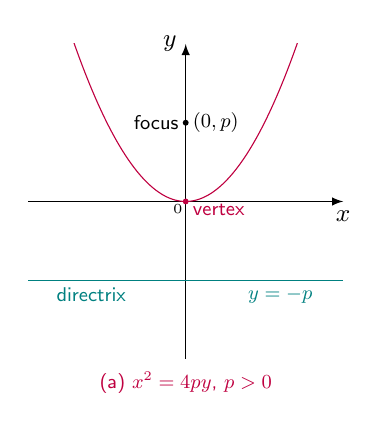
\begin{tikzpicture}[>=latex,xscale=.5*1, yscale=.5*1][font=\sf\small]

\draw[->] (-4, 0) -- (4, 0)node[below] {\small $x$};
\draw[->] (0, -4) -- (0, 4)node[left] {\small $y$};

\node[purple, scale=0.8] at (0, -4.6) {(a) $x^2 = 4py$, $p > 0$};

\clip[] (-4,-4) rectangle (4,4);

\draw[purple, samples=100, smooth, domain=-3:3, variable=\x]
plot ({\x}, {1/4*2*(\x)^2}) ;

\draw[teal] (-4,-2) -- (4, -2) node[below, pos=0.2, scale=0.8]{$\hbox{directrix}$} node[below, pos=0.8, scale=0.8]{$y=-p$};

\draw[fill] (0, 2) circle(0.06) node[left, scale=0.8]{$\hbox{focus}$} node[right, scale=0.8]{$(0, p)$};

\draw[purple, fill] (0, 0) circle(0.06)node[right, yshift=-3, scale=0.8]{$\hbox{vertex}$};

\node at (-0.2/1, -0.2/1) {\tiny$0$};

\end{tikzpicture}\hskip1cm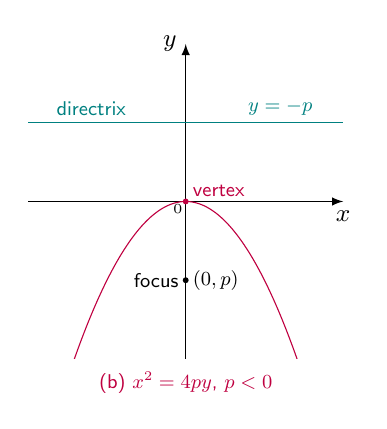
\begin{tikzpicture}[>=latex,xscale=.5*1, yscale=.5*1][font=\sf\small]

\draw[->] (-4, 0) -- (4, 0)node[below] {\small $x$};
\draw[->] (0, -4) -- (0, 4)node[left] {\small $y$};

\node[purple, scale=0.8] at (0, -4.6) {(b) $x^2 = 4py$, $p < 0$};

\clip[] (-4,-4) rectangle (4,4);

\draw[purple, samples=100, smooth, domain=-3:3, variable=\x]
plot ({\x}, {-1/4*2*(\x)^2}) ;

\draw[teal] (-4, 2) -- (4, 2) node[above, pos=0.2, scale=0.8]{$\hbox{directrix}$} node[above, pos=0.8, scale=0.8]{$y=-p$};

\draw[fill] (0, -2) circle(0.06) node[left, scale=0.8]{$\hbox{focus}$} node[right, scale=0.8]{$(0, p)$};

\draw[purple, fill] (0, 0) circle(0.06)node[right, yshift= 4, scale=0.8]{$\hbox{vertex}$};

\node at (-0.2/1, -0.2/1) {\tiny$0$};

\end{tikzpicture}
\end{document}